\subsection{Radiation Monitoring System}
\label{sec:RadiationDesign}

\subsubsection{MiniPIX Detector}
The MiniPIX detector is a silicon-based hyrbid pixel detector founded on Timepix technology. The device is built by ADVACAM \cite{Advacam}  and utilizes technology developed by the Medipix Collaboration at CERN \cite{Medipix}. The sensor consists of a \num{256}x\num{256} array of pixels and a pitch of \SI{55}{\micro\meter}. A USB 2.0 connection is used to interface with the device, which provides power and data output. The primary use of the detector will be to characterize cosmic radiation by the type of particle and its incident energy.
%The device is capable of operating in the following three different modes: single particle counting, Time-over-Threshold, and Time-of-Arrival.

\begin{figure}[H]
  \begin{minipage}[c]{0.40\linewidth}
    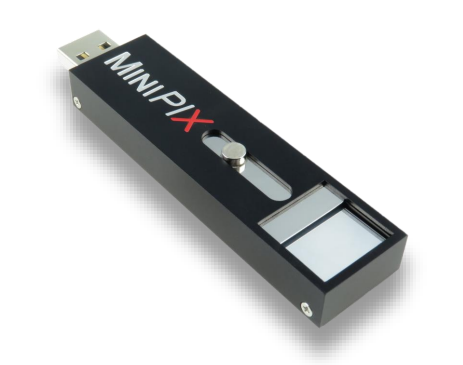
\includegraphics[width=\linewidth]{Figures/Minipix2.png}
    \caption{Picture of a MiniPIX particle detector~\cite{Advacam}.}
    \label{fig:Minipix}
  \end{minipage}
  \hfill
  \begin{minipage}[c]{0.45\linewidth}
    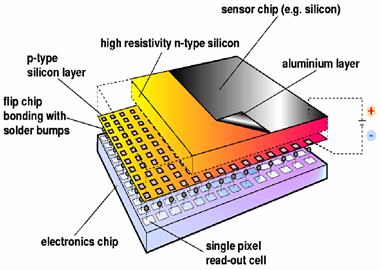
\includegraphics[width=\linewidth]{Figures/MinipixLayers.png}
    \caption{Layers that makeup the MiniPIX sensor.}
    \label{fig:MinipixLayers}
  \end{minipage}
\end{figure}

When an ionizing particle hits the sensor, electron-hole pairs accumulate within the semiconducting material. The electronics reads-out the pairs by depleting the silicon with a bias voltage. If a charge is above the set threshold, the charge is counted. The energy deposited in a pixel can be determined from the back-plane pulse amplitude. Particles incident on the sensor appear as pixel clusters, which is defined as a continuous area of activated pixels. By analyzing these clusters, the incident particle can be identified. The morphology of the cluster gives information regarding the type of particle as well as the angle at which the particle was incident upon the detector. 

Detectors using Timepix technology are used to measure radiation aboard the ISS. Since the University of Houston is a member of the Medipix Collaboration, scientists at the University of Houston work with preparing Medpix devices to be used aboard the ISS. As a result, the UH HASP team may be able to work with these scientists and compare data gathered from the mockup ISS module to data from the ISS.

Due to the SORA 3 mission being a continuation of previous missions, we have the opportunity to compare data from previous flights. For example, this will allow us to observe how data regarding particle counts and dose changes with the solar cycle. Hathaway \cite{Hathaway} has shown that a direct relationship exists between the development of the solar cycle and neutron counts.

\begin{figure}[h]
    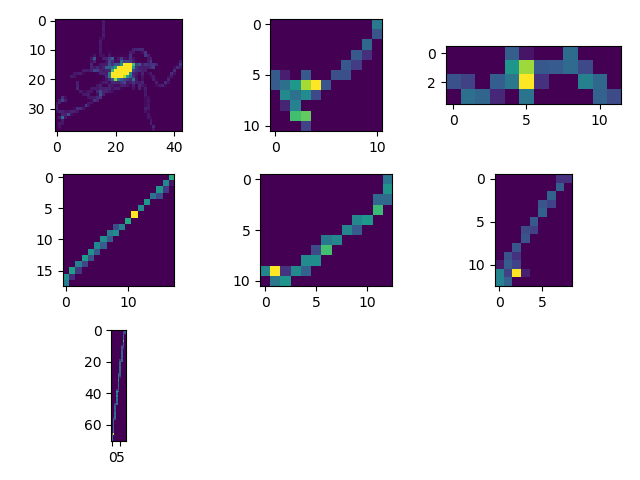
\includegraphics[scale=1, width=.75\textwidth]{Figures/Tracks.png}
    \caption{Examples of different track types from data collected by a MiniPIX.}
    \label{fig:Tracks}
\end{figure}

\subsubsection{Calibration}   
It is necessary to calibrate the sensor. The calibration procedure is rather sophisticated, so the calibration will be applied by Dr. Stuart P. George at the University of Houston. Dr. George is a member of the Medipix Collaboration. The general outline of the calibration is as follows. A source calibration is applied by using a \SI{60}{\keV}{\ce{^241Am} decary line, \ce{Sn} Flourescence and \ce{^55Fe} gamma rays. The pixel detector consists of \num{65536} silicon p-n dioded, each containing its own individual processing circuit. The response of each pixel can never to identical to one another, so a calibration mut be performed on each pixel. Dr. George will calibrate each pixel energy threshold from DAC counts to energy \cite{StuartThesis}. The threshold of the sensor will be set to \SI{4}{\keV}, which sufficiently filters out background noise. The bias voltage of the sensor will be set to \SI{200}{\volt}, which guarantees that the silicon is completely depleted while reading out the charge.
  
\subsubsection{Collection Parameters}
% Put the settings for the minipix shutter time, bias voltage etc. here
ADVACAM has developed a Python API to configure the device and its acquisition parameters. The shutter speed of the device controls the rate at which data is output from the device. The shutter speed controls the exposure time of the sensor before saving the data to a frame. Once the data is saved, the device enters manufacturer-set dormant period, which lasts for approximately two seconds. This time will be utilized as a cool-down period for the device. The value of the shutter speed is highly dependent on the application of the sensor. Within the context of HASP, we expect high radiation exposure which will require a quicker shutter speed. This is to the fact that if the shutter speed is too long, the sensor become overcrowded and clusters become difficult or impossible to analyze. However, if the shutter speed is too short, there will be many frames with little to no data, which will use a large amount of storage space. Based off of previous SORA missions, a shutter speed of a few seconds is sufficient for our application. The exact shutter speed will be determined through testing and may be different for each device we use.

\subsubsection{Data Format}
The data frames are stored as plain text values where each value corresponds to a value from a pixel on the pixel array. In a separate file, metadata such as acquisition type, shutter speed, bias voltage, and other parameters are recorded for each frame. Both the data file and the metadata file will be stored on the RP\num{3} and the various redundant storage systems we implement. The MiniPIX data from previous missions used about \SIrange{1}{2}{\giga\byte}. For the 2019 mission, we expect about double that value due to our use of two MiniPIX devices.

\subsubsection{Structure}
The MiniPIX outside of the ISS module will be contained within a small case plastic case to protect the device from atmospheric moisture. Thermal paste will be used to fix the MiniPIX on a small block of aluminum, which will behave as a heat sink. This simple setup has proven to work on previous missions and is shown in Figure \ref{fig:CaseAssembly}.
\begin{figure}[h]
    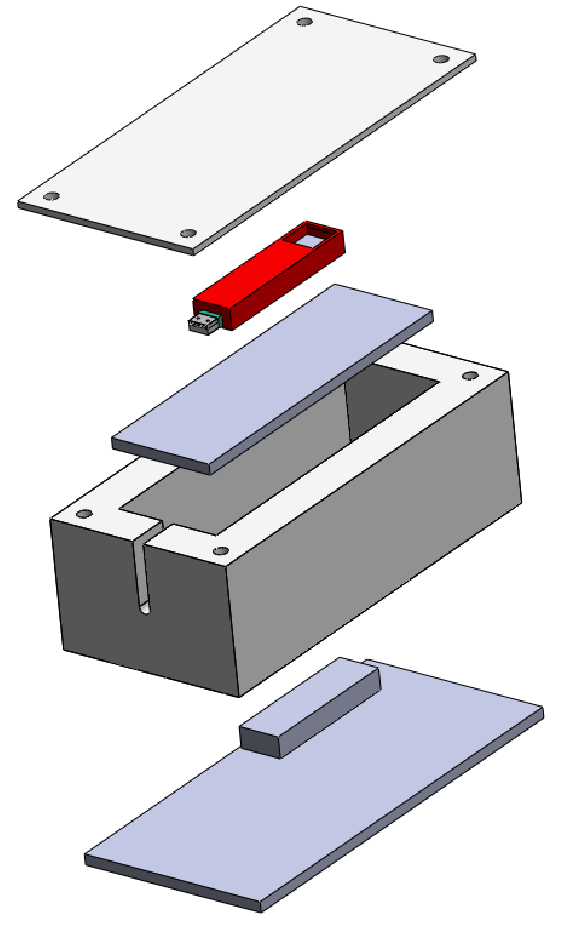
\includegraphics[scale=1, width=.25\textwidth]{Figures/MinipixCaseAssembly.pdf}
    \caption{Examples of different track types from data collected by a MiniPIX.}
    \label{fig:CaseAssembly}
\end{figure}

\subsubsection{ISS Module}
\label{subsec:ISSModule}
As part of the radiation subsystem, the payload will include a capsule intended to mimic the structure of one of NASA's modules on the ISS.
The method deployed by NASA and other agencies is called ``Stuffed Whipple'' shielding and is deployed in ISS modules that are at highest risk of impact \cite{NASAShielding}.
This module will remain at atmospheric pressure throughout the entire flight in attempt to model the environment as closely as possible.
Inside the capsule will be a scintillated MiniPIX that will record the radiation environment within the module.
The scintillated MiniPIX will measure the neutrons within the ISS structure in attempt to determine the exposure within the structure.

The materials that make-up the module will be those used in the outer walls on the ISS and will have the same thickness.
The main differences in structure will be the lack of standoffs and the lack of a multi-layer insulator (MLI) in our module.
The walls of the ISS have standoffs between layers of materials, which increases the total wall thickness to about one foot.
Additionally, the MLI used by NASA is not available commercially.
%Due to being in space, the gaps between the layers are a vacuum.
In the interest of saving space, we will not include the standoffs, and all materials will be layered on one another in the same order as they are used on the ISS.

\begin{figure}[H]
  \centering
  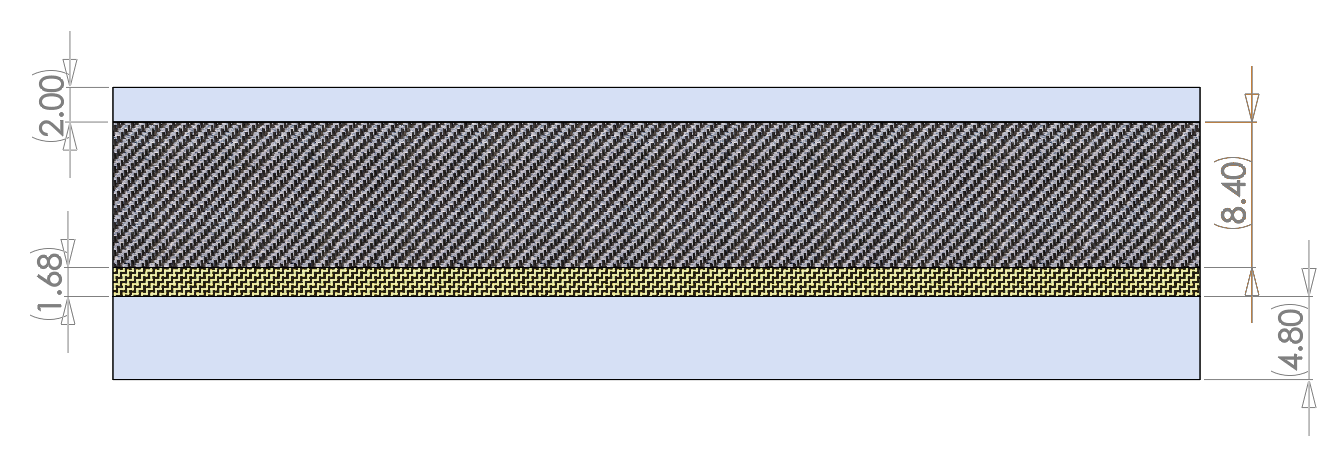
\includegraphics[width=0.8\linewidth]{Figures/MaterialCrossSection.png}
  \caption{Layers and thicknesses of the materials that will be used to construct the ISS module. From top to bottom: aluminum 6061-T6, six layers of Nextel AF62, six layers of Kevlar fabric, and aluminum 2219-T87. The atmosphere is contained by the \SI{4.8}{\milli\meter} layer of aluminum \cite{NASAPP}. All measurements are in \si{\milli\meter}.} 
  \label{fig:ISSLayers}
\end{figure}

%To construct the module, a rectangular box of aluminum will be constructed with one missing face, constituting the inner aluminum box that will contain the pressurized environment. The 

\subsubsection{Scintillated MiniPIX}
The MiniPIX's sensor can only interact with charged particles. In order to measure neutrons with the MiniPIX, a scintillator is rerquired. The scintillator will interact with the neutrons and produce a specific signature of particles which can be measured by the MiniPIX. Uher et al. \cite{Uher} used a similar method, but with a lithium-based scintillator. We will use a boron-loaded plastic scintillator \cite{BoronScintillator} to cover exactly half of the MiniPIX sensor. The reation between the Boron-10 nucleus and a thermal neutron is \[\ce{^10B + n -> ^7Li + ^4He + \gamma (\SI{480}{\kilo\eV})}\] according to Pawelczak et al \cite{Pawelczak}. This scintillator was chosen due to its large reaction cross-section for thermal neutron capture and its emission of light charged particles. This larger rwaction cross-section increases the probability that the neutron will produce particles that can be measured by the MiniPIX.

By covering half of the sensor, we can compare the uncovered half with the data recorded by the MiniPIX outside of the ISS module.

\subsubsection{Organic Photovoltaic Cells}    
We will be using four different types of solar cells with a total of 12 arrays on board our payload. There will be one type of cell on each of three sides of the payload, leaving one face free for any unique cells we may develop during our research. Half of our panels will be prefabricated and purcahsed from a supplier, and will be regarded as a control against which we will evaluate our in house fabricated cells. For the in house fabrication, we will be focusing on polymer:fullerne BHJ and perovskite active layer cells. We intend to investigate a variety of polymer:fullerene blends and develop a procedue for fabrication which yields the greatest PCE and MPP in the stratospheric environment, and to investigate the possibility of transpatent conductive oxide(TCO) layers besides the traditional indium tin oxide (ITO) glass and polyethylene terephthalate (PET) plastic. 

Solar cells are characterized by their current vs voltage (IV) curve, which tells you the maximum power point (MPP), Vmax and Imax, open-circuit voltage (Voc) and short circuit current (Isc), leading to the fill factor (FF) and efficiency (PCE). This curve will be  generated using a variable resistor in series with two multimeters, one acting as voltmeter and the other an ammeter, and the solar cell in question, which will follow Ohm's law (1) V=IR. From the plot, Voc is seen when I=0, Isc is when V=0, and the MPP is where Vmax and Imax meet. The MPP can then tell us the efficiecy, which is defined as (2) MPP/Pin. The fill factor gives information on the "squarness" of the IV curve and is defined as (3) FF = MPP/VocIsc, and it is optimal to maximize the fill factor. \cite{OPV operation}

    Before flight, every cell will be characterized with IV curves using AMG 0 simulated sun light to generate a characteristic profile, as expected in the space environment, for the each new cell, and microscopy will be preformed to understand the topology and interfacial details of the new cells. Currently our plan is to have one of each cell type remaining on ground as a control, and we will have each panel onboard the payload wired to an arduino unit where IV curves will be recorded during flight, with a characteristic profile generated every 30 seconds. This data will be stored on the arduino with backup stored to a raspberry pi. On  board our payload we will be measuring the tempreature and pressure of the environment to deteremaine any effects on the preformance due to temperature and pressure changes. Finally after recovery, the IV data will be extracted from the arduino/raspberry pi and plotted, and each cell will be re characterized and once again viewed under the microscope to look for any physical defects. 
    
    With the HASP mission, we are going to compare fabricated organic polymer and perovskite solar cells against purchased prefabricated organic solar cells. Each of these cells will be analyzed before, during, and after exposure to the stratosphere. In analyzing our cells, we will measure the open circuit voltage, short circuit current, and maiximum power point, then fill factor will be determined along with efficieny.
    In conjunction with our MiniPIX detector, we will be analyzing the effect that cosmic ray bombardment has on our solar cells. By analyzing the times at which cosmic rays are recorded, we can look at our IV data and determine if there was any effect on the cells preformance. Additionally, we will watch for problems which arise due to UV-A, B, and C rays with photodiodes. These photodiodes will serve the additional purpose of monitoring the solar power spectrum that our cells are exposed to.
    


